\documentclass[tikz]{standalone}

% tikz
\usepackage{tikz, pgfplots}
% i wish external worked but idk it sucks
%\usetikzlibrary{external}
%\tikzexternalize[prefix=figures/]

% for function graph
\usetikzlibrary{positioning}
\usetikzlibrary{shapes.geometric}
\usetikzlibrary{positioning}
\tikzset{
dot/.style = {circle, fill=#1, minimum size=5pt,
              inner sep=0pt, outer sep=0pt},
dot/.default = black % size of the circle diameter
}

 % for braces
\usetikzlibrary{decorations.pathreplacing}
% for hashing area
\usetikzlibrary{patterns}
% tableaux var, signe
% source https://www.sqlpac.com/fr/documents/latex-package-tkz-tab-tikz-tableaux-de-signes-et-de-variations-de-fonctions.html
\usepackage{tkz-tab}
%%%%%%%%%%%%%%%%%%%%%%%%%%%%%%
% SELF MADE COLORS
%%%%%%%%%%%%%%%%%%%%%%%%%%%%%%


\definecolor{myg}{RGB}{56, 140, 70}
\definecolor{myb}{RGB}{45, 111, 177}
\definecolor{myr}{RGB}{199, 68, 64}
\definecolor{mytheorembg}{HTML}{F2F2F9}
\definecolor{mytheoremfr}{HTML}{00007B}
\definecolor{mylenmabg}{HTML}{FFFAF8}
\definecolor{mylenmafr}{HTML}{983b0f}
\definecolor{mypropbg}{HTML}{f2fbfc}
\definecolor{mypropfr}{HTML}{191971}
\definecolor{myexamplebg}{HTML}{F2FBF8}
\definecolor{myexamplefr}{HTML}{88D6D1}
\definecolor{myexampleti}{HTML}{2A7F7F}
\definecolor{mydefinitbg}{HTML}{E5E5FF}
\definecolor{mydefinitfr}{HTML}{3F3FA3}
\definecolor{notesgreen}{RGB}{0,162,0}
\definecolor{myp}{RGB}{197, 92, 212}
\definecolor{mygr}{HTML}{2C3338}
\definecolor{myred}{RGB}{127,0,0}
\definecolor{myyellow}{RGB}{169,121,69}
\definecolor{myexercisebg}{HTML}{F2FBF8}
\definecolor{myexercisefg}{HTML}{88D6D1}
\definecolor{doc}{RGB}{0,60,110}

% manim colors because they're beautiful
% https://docs.manim.community/en/stable/reference/manim.utils.color.manim_colors.html

\definecolor{BLACK}{HTML}{000000}\definecolor{BLUE}{HTML}{58C4DD}\definecolor{BLUE_A}{HTML}{C7E9F1}\definecolor{BLUE_B}{HTML}{9CDCEB}\definecolor{BLUE_C}{HTML}{58C4DD}\definecolor{BLUE_D}{HTML}{29ABCA}\definecolor{BLUE_E}{HTML}{236B8E}\definecolor{DARKER_GRAY}{HTML}{222222}\definecolor{DARKER_GREY}{HTML}{222222}\definecolor{DARK_BLUE}{HTML}{236B8E}\definecolor{DARK_BROWN}{HTML}{8B4513}\definecolor{DARK_GRAY}{HTML}{444444}\definecolor{DARK_GREY}{HTML}{444444}\definecolor{GOLD}{HTML}{F0AC5F}\definecolor{GOLD_A}{HTML}{F7C797}\definecolor{GOLD_B}{HTML}{F9B775}\definecolor{GOLD_C}{HTML}{F0AC5F}\definecolor{GOLD_D}{HTML}{E1A158}\definecolor{GOLD_E}{HTML}{C78D46}\definecolor{GRAY}{HTML}{888888}\definecolor{GRAY_A}{HTML}{DDDDDD}\definecolor{GRAY_B}{HTML}{BBBBBB}\definecolor{GRAY_BROWN}{HTML}{736357}\definecolor{GRAY_C}{HTML}{888888}\definecolor{GRAY_D}{HTML}{444444}\definecolor{GRAY_E}{HTML}{222222}\definecolor{GREEN}{HTML}{83C167}\definecolor{GREEN_A}{HTML}{C9E2AE}\definecolor{GREEN_B}{HTML}{A6CF8C}\definecolor{GREEN_C}{HTML}{83C167}\definecolor{GREEN_D}{HTML}{77B05D}\definecolor{GREEN_E}{HTML}{699C52}\definecolor{GREY}{HTML}{888888}\definecolor{GREY_A}{HTML}{DDDDDD}\definecolor{GREY_B}{HTML}{BBBBBB}\definecolor{GREY_BROWN}{HTML}{736357}\definecolor{GREY_C}{HTML}{888888}\definecolor{GREY_D}{HTML}{444444}\definecolor{GREY_E}{HTML}{222222}\definecolor{LIGHTER_GRAY}{HTML}{DDDDDD}\definecolor{LIGHTER_GREY}{HTML}{DDDDDD}\definecolor{LIGHT_BROWN}{HTML}{CD853F}\definecolor{LIGHT_GRAY}{HTML}{BBBBBB}\definecolor{LIGHT_GREY}{HTML}{BBBBBB}\definecolor{LIGHT_PINK}{HTML}{DC75CD}\definecolor{LOGO_BLACK}{HTML}{343434}\definecolor{LOGO_BLUE}{HTML}{525893}\definecolor{LOGO_GREEN}{HTML}{87C2A5}\definecolor{LOGO_RED}{HTML}{E07A5F}\definecolor{LOGO_WHITE}{HTML}{ECE7E2}\definecolor{MAROON}{HTML}{C55F73}\definecolor{MAROON_A}{HTML}{ECABC1}\definecolor{MAROON_B}{HTML}{EC92AB}\definecolor{MAROON_C}{HTML}{C55F73}\definecolor{MAROON_D}{HTML}{A24D61}\definecolor{MAROON_E}{HTML}{94424F}\definecolor{ORANGE}{HTML}{FF862F}\definecolor{PINK}{HTML}{D147BD}\definecolor{PURE_BLUE}{HTML}{0000FF}\definecolor{PURE_GREEN}{HTML}{00FF00}\definecolor{PURE_RED}{HTML}{FF0000}\definecolor{PURPLE}{HTML}{9A72AC}\definecolor{PURPLE_A}{HTML}{CAA3E8}\definecolor{PURPLE_B}{HTML}{B189C6}\definecolor{PURPLE_C}{HTML}{9A72AC}\definecolor{PURPLE_D}{HTML}{715582}\definecolor{PURPLE_E}{HTML}{644172}\definecolor{RED}{HTML}{FC6255}\definecolor{RED_A}{HTML}{F7A1A3}\definecolor{RED_B}{HTML}{FF8080}\definecolor{RED_C}{HTML}{FC6255}\definecolor{RED_D}{HTML}{E65A4C}\definecolor{RED_E}{HTML}{CF5044}\definecolor{TEAL}{HTML}{5CD0B3}\definecolor{TEAL_A}{HTML}{ACEAD7}\definecolor{TEAL_B}{HTML}{76DDC0}\definecolor{TEAL_C}{HTML}{5CD0B3}\definecolor{TEAL_D}{HTML}{55C1A7}\definecolor{TEAL_E}{HTML}{49A88F}\definecolor{WHITE}{HTML}{FFFFFF}\definecolor{YELLOW}{HTML}{FFFF00}\definecolor{YELLOW_A}{HTML}{FFF1B6}\definecolor{YELLOW_B}{HTML}{FFEA94}\definecolor{YELLOW_C}{HTML}{FFFF00}\definecolor{YELLOW_D}{HTML}{F4D345}\definecolor{YELLOW_E}{HTML}{E8C11C}

% Schwartz
\renewcommand{\S}{\mathcal{S}} % \S est le signe paragraphe normalement

% corps
\newcommand{\C}{\mathcal{C}}
\newcommand{\R}{\mathbb{R}}
\newcommand{\Rnn}{\mathbb{R}^{2n}}
\newcommand{\Z}{\mathbb{Z}}
\newcommand{\N}{\mathbb{N}}
\newcommand{\Q}{\mathbb{Q}}

% domain
\newcommand{\D}{\mathcal{D}}

% order notations
\renewcommand{\O}{\mathcal{O}}

% japanese bracket
\newcommand{\japb}[1]{\langle #1 \rangle}

% arrows over partial derivatives
\newcommand{\lp}{\overleftarrow{\partial}}
\newcommand{\rp}{\overrightarrow{\partial}}

% quantization
\newcommand{\h}{\hbar}
\newcommand{\Opht}{\textrm{Op}_{\h}^{t}}
\newcommand{\Op}[2][\hbar]{\textrm{Op}_{#1}^{#2}}

% omega functions
\newcommand{\omegap}[2][\rho_0]{\omega(\partial_{#1},\partial_{#2})}
\newcommand{\omegar}[2][\rho_0]{\omega(#1,#2)}

\tikzset{
	every node/.style = {font=\Large}
}

\tikzset{
	every axis/.style = {clip=false, grid style = {opacity=.5}}
}

\begin{document}
%
	% page 1
	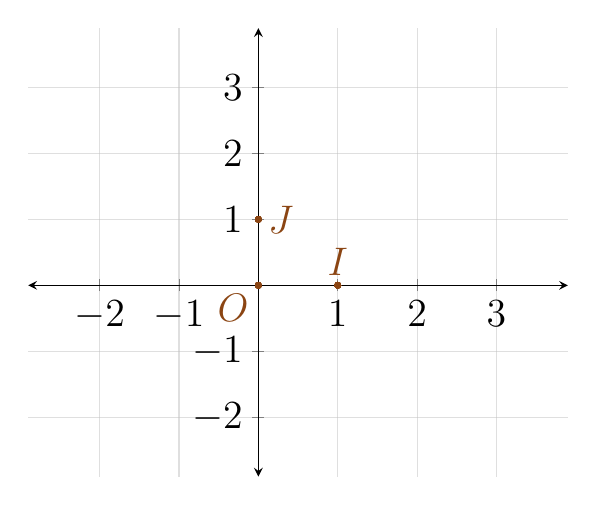
\begin{tikzpicture}[>=stealth, scale=1]
		\begin{axis}[xmin = -2.9, xmax=3.9, xtick={ -3, ..., 5}, ymin=-2.9, ymax=3.9, ytick={-3, ..., 5}, axis x line=middle, axis y line=middle, axis line style=<->, xlabel={}, ylabel={}, grid=both, grid style = {opacity=.5}]
		
			\addplot[DARK_BROWN, mark=*, mark size = 1] (0,0) node[below=8pt, left] {$O$};
			\addplot[DARK_BROWN, mark=*, mark size = 1] (1,0) node[above] {$I$};
			\addplot[DARK_BROWN, mark=*, mark size = 1] (0,1) node[right] {$J$};
		\end{axis}
	\end{tikzpicture}
	
	% page 2
	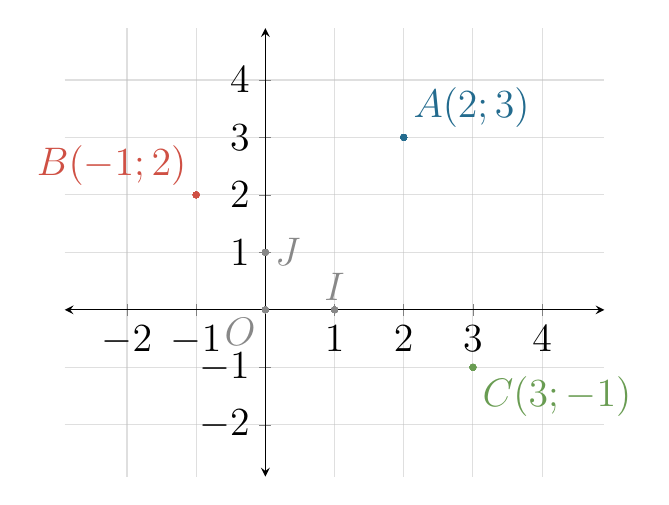
\begin{tikzpicture}[>=stealth, scale=1]
		\begin{axis}[xmin = -2.9, xmax=4.9, xtick={ -3, ..., 5}, ymin=-2.9, ymax=4.9, ytick={-3, ..., 5}, axis x line=middle, axis y line=middle, axis line style=<->, xlabel={}, ylabel={}, grid=both, grid style = {opacity=.5}]
		
			\addplot[GREY, mark=*, mark size = 1] (0,0) node[below=8pt, left] {$O$};
			\addplot[GREY, mark=*, mark size = 1] (1,0) node[above] {$I$};
			\addplot[GREY, mark=*, mark size = 1] (0,1) node[right] {$J$};
			
			\addplot[BLUE_E, mark=*, mark size = 1] (2,3) node[above right] {$A(2 ; 3)$};
			\addplot[RED_E, mark=*, mark size = 1] (-1,2) node[above left] {$B(-1 ; 2)$};
			\addplot[GREEN_E, mark=*, mark size = 1] (3,-1) node[below right] {$C(3; -1)$};
		\end{axis}
	\end{tikzpicture}
	
	% page 3
	\begin{tikzpicture}[>=stealth, scale=1.2]
		\begin{axis}[xmin = -6.9, xmax=22.9, xticklabel=\empty, ymin=-2.9, ymax=4.9, yticklabel=\empty, axis x line=middle, axis y line=middle, axis line style=<->, xlabel={}, ylabel={},  ticks=none, clip=false, x=10pt]
		
			% A and B
			\addplot[black, mark=*, mark size = 1] (1,3) node[above right] {$A({\color{PURPLE_E}x_A}; {\color{RED_E}y_A})$};
			\addplot[black, mark=*, mark size = 1] (20,-2) node[below right] {$B({\color{PURPLE_E}x_B}; {\color{RED_E}y_B})$};
			
			
			\addplot[PURPLE_E, very thick, mark=|, mark size = 2] (1,-.07) node[below] {$x_A$};
			\addplot[PURPLE_E, very thick, mark=|, mark size = 2] (20,.07) node[above] {$x_B$};
			\addplot[RED_E,very thick, mark=-, mark size = 2] (-.2,3) node[left] {$y_A$};
			\addplot[RED_E, very thick, mark=-, mark size = 2] (-.2,-2) node[left] {$y_B$};
			
			% midpoint
			\addplot[black, mark=*, mark size = 1] (10.5,.5) node[above right] {$M$};	
			
			\addplot[PURPLE_E, very thick, mark=|, mark size = 2] (10.5,-.07) node[below=3pt] {$\dfrac{x_A+x_B}2$};
			\draw[PURPLE_E, dashed, very thick] (axis cs:10.5, 0) -- (axis cs:10.5,.5);
			
			\addplot[RED_E, very thick, mark=-, mark size = 2] (-.2,.5) node[above=3pt, left] {$\dfrac{y_A+y_B}2$};
			\addplot[RED_E, dashed, very thick, domain = 0:10.5, samples=2] {.5};			
			
			% dashed rectangle
			\draw[PURPLE_E, dashed, very thick] (axis cs:1, 0) -- (axis cs:1,3);
			\draw[PURPLE_E, dashed, very thick] (axis cs:20, 0) -- (axis cs:20,-2);
			\addplot[RED_E, dashed, very thick, domain = 0:1, samples=2] {3};
			\addplot[RED_E, dashed, very thick, domain = 0:20, samples=2] {-2};
			
			% formula
			%\addplot[black] (15,3) node[right, draw] {$M = \dfrac{A+B}2$};
			\addplot[black] (12,3) node[right, draw] {$M\Bigl({\color{PURPLE_E}\dfrac{x_A+x_B}2} ; {\color{RED_E}\dfrac{y_A+y_B}2}\Bigr)$};
			
			% [AB]
			
			\draw[-, black, dotted, thin] (axis cs:1,3) -- (axis cs:20,-2);
			
		\end{axis}
	\end{tikzpicture}
	
	% page 4
	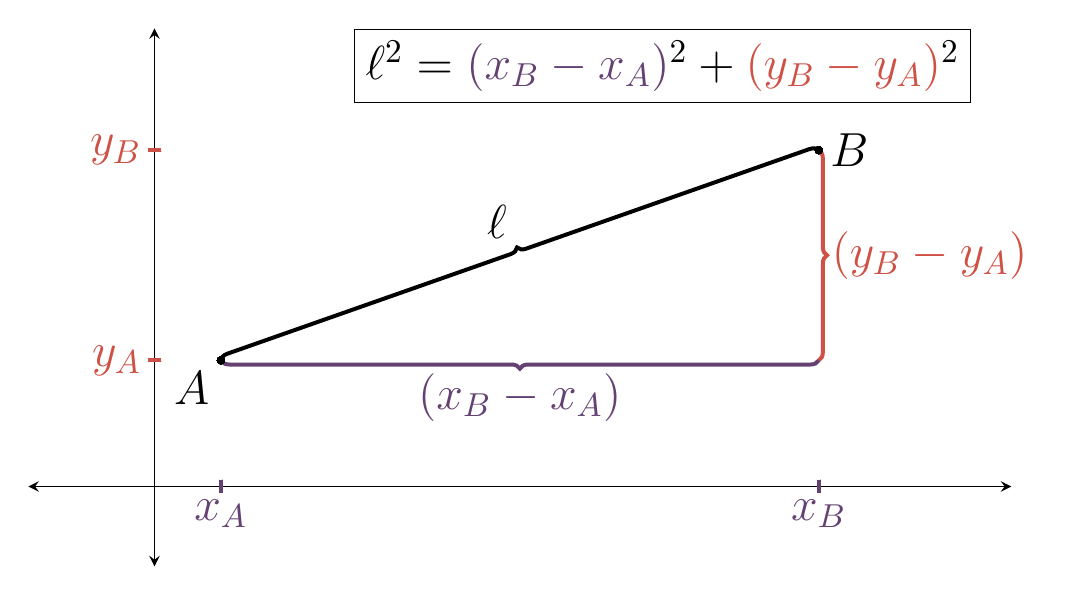
\begin{tikzpicture}[>=stealth, scale=1.2]
		\begin{axis}[xmin = -1.9, xmax=12.9, xticklabel=\empty, ymin=-1.9, ymax=10.9, yticklabel=\empty, axis x line=middle, axis y line=middle, axis line style=<->, xlabel={}, ylabel={}, ticks=none, clip=false, x=20pt]
		
			% A and B
			\addplot[black, mark=*, mark size = 1] (1,3) node[below left] {$A$};
			\addplot[black, mark=*, mark size = 1] (10,8) node[right] {$B$};
			
			
			\addplot[PURPLE_E, mark=|, mark size = 2, very thick] (1,0) node[below] {$x_A$};
			\addplot[PURPLE_E, mark=|, mark size = 2, very thick] (10,0) node[below] {$x_B$};
			\addplot[RED_E, mark=-, mark size = 2, very thick] (0,3) node[left] {$y_A$};
			\addplot[RED_E, mark=-, mark size = 2, very thick] (0,8) node[left] {$y_B$};
			
			% triangle
			\draw[RED_E, very thick, decorate, decoration = {brace, mirror}] (axis cs:10,3) -- (axis cs:10,8) node [midway, right]{$(y_B - y_A)$};
			\draw[black, very thick, decorate, decoration = {brace}] (axis cs:1, 3) -- (axis cs:10,8) node [midway, above=10pt, left]{$\ell$};
			\draw[PURPLE_E, very thick, decorate, decoration = {brace, mirror}] (axis cs:1, 3) -- (axis cs:10,3) node [midway, below]{$(x_B-x_A)$};
			
			% formula
			\addplot[black] (3,10) node[right, draw] {$\ell^2 = {\color{PURPLE_E}(x_B-x_A)}^2 + {\color{RED_E}(y_B - y_A)}^2$};
			
		\end{axis}
	\end{tikzpicture}
	% exe:points-à-placer 
	% page 5
	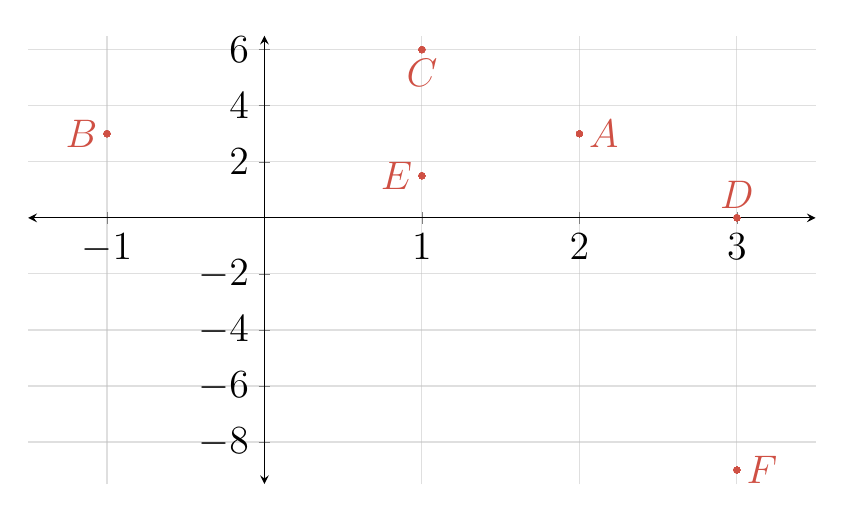
\begin{tikzpicture}[>=stealth, scale=1]
		\begin{axis}[xmin = -1.5, xmax=3.5, ymin=-9.5, ymax=6.5, ytick = {-8, -6, ..., 6}, xtick = {-1, 0, ..., 3}, axis x line=middle, axis y line=middle, axis line style=<->, xlabel={}, ylabel={}, grid=both, x=2cm]
						
			\addplot[RED_E, mark=*, mark size = 1] (2,3) node[right] {$A$};
			\addplot[RED_E, mark=*, mark size = 1] (-1,3) node[left] {$B$};
			\addplot[RED_E, mark=*, mark size = 1] (1,6) node[below] {$C$};
			\addplot[RED_E, mark=*, mark size = 1] (3,0) node[above] {$D$};
			\addplot[RED_E, mark=*, mark size = 1] (1,1.5) node[left] {$E$};
			\addplot[RED_E, mark=*, mark size = 1] (3,-9) node[right] {$F$};
			
		\end{axis}
	\end{tikzpicture}
	
	% exe:prénom
	% page 6
	\begin{tikzpicture}[>=stealth, scale=1]
		\begin{axis}[xmin = -.1, xmax=2.1, xtick={ -3, ..., 5}, ymin=-.1, ymax=3.1, ytick={-3, ..., 5}, axis x line=middle, axis y line=middle, axis line style=<->, xlabel={}, ylabel={}, grid=both, grid style = {opacity=.5}, clip=false, x=5cm]
			
			\addplot[BLUE_E, mark=*, mark size = 1] (0,0) node[above left] {$A(0;0)$};
			\addplot[RED_E, mark=*, mark size = 1] (0,3) node[above left] {$B(0;3)$};
			\addplot[GREEN_E, mark=*, mark size = 1] (1,2) node[below] {$C(1;2)$};
			\addplot[BLUE_E, mark=*, mark size = 1] (2,3) node[above right] {$D(2;3)$};
			\addplot[RED_E, mark=*, mark size = 1] (2,0) node[above right] {$E(2;0)$};
			
			\draw[-, thick,dashed] (axis cs:0,0) -- (axis cs:0,3);
			\draw[-, thick, dashed] (axis cs:0,3) -- (axis cs:1,2);
			\draw[-, thick,dashed] (axis cs:1,2) -- (axis cs:2,3);
			\draw[-, thick,dashed] (axis cs:2,3) -- (axis cs:2,0);
		\end{axis}
	\end{tikzpicture}
	
	% exe:lecture-coord
	% page 7
	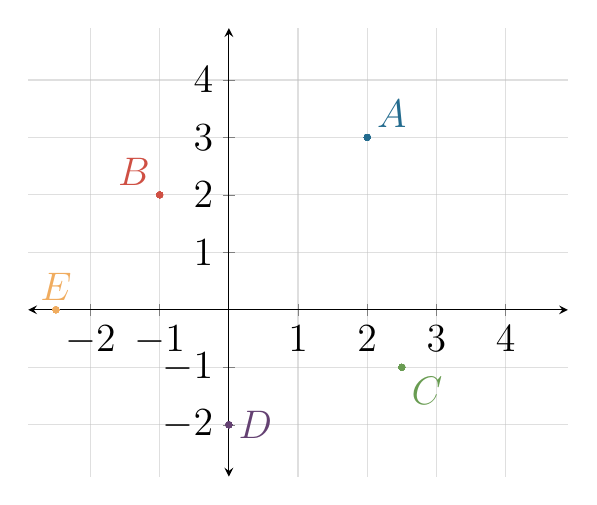
\begin{tikzpicture}[>=stealth, scale=1]
		\begin{axis}[xmin = -2.9, xmax=4.9, xtick={ -3, ..., 5}, ymin=-2.9, ymax=4.9, ytick={-3, ..., 5}, axis x line=middle, axis y line=middle, axis line style=<->, xlabel={}, ylabel={}, grid=both, grid style = {opacity=.5}]			
			\addplot[BLUE_E, mark=*, mark size = 1] (2,3) node[above right] {$A$};
			\addplot[RED_E, mark=*, mark size = 1] (-1,2) node[above left] {$B$};
			\addplot[GREEN_E, mark=*, mark size = 1] (2.5,-1) node[below right] {$C$};
			\addplot[PURPLE_E, mark=*, mark size = 1] (0,-2) node[right] {$D$};
			\addplot[GOLD, mark=*, mark size = 1] (-2.5,0) node[above] {$E$};
		\end{axis}
	\end{tikzpicture}
	
	% exe:Trex
	% page 8
	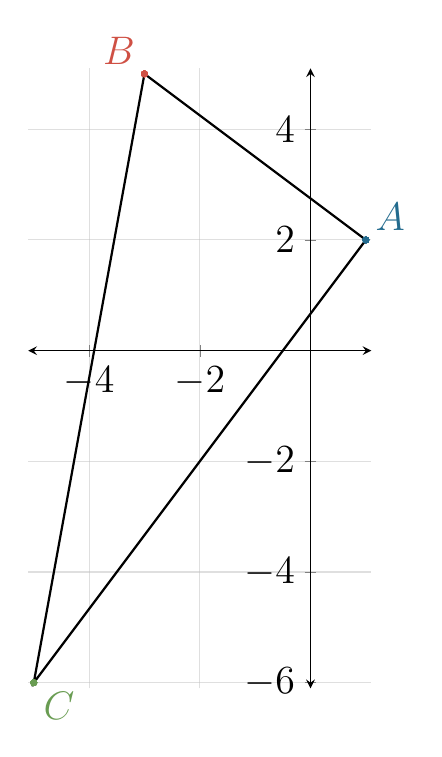
\begin{tikzpicture}[>=stealth, scale=1]
		\begin{axis}[xmin = -5.1, xmax=1.1, ymin=-6.1, ymax=5.1,axis x line=middle, axis y line=middle, axis line style=<->, xlabel={}, ylabel={}, grid=both, grid style = {opacity=.5}, x=20pt, y=20pt]
			\addplot[BLUE_E, mark=*, mark size = 1] (1,2) node[above right] {$A$};
			\addplot[RED_E, mark=*, mark size = 1] (-3,5) node[above left] {$B$};
			\addplot[GREEN_E, mark=*, mark size = 1] (-5,-6) node[below right] {$C$};
			
			\draw[-, thick] (axis cs:1,2) -- (axis cs:-3,5) -- (axis cs:-5,-6) -- (axis cs:1,2);
		\end{axis}
	\end{tikzpicture}
	
	% exe:C03
	% page 9
	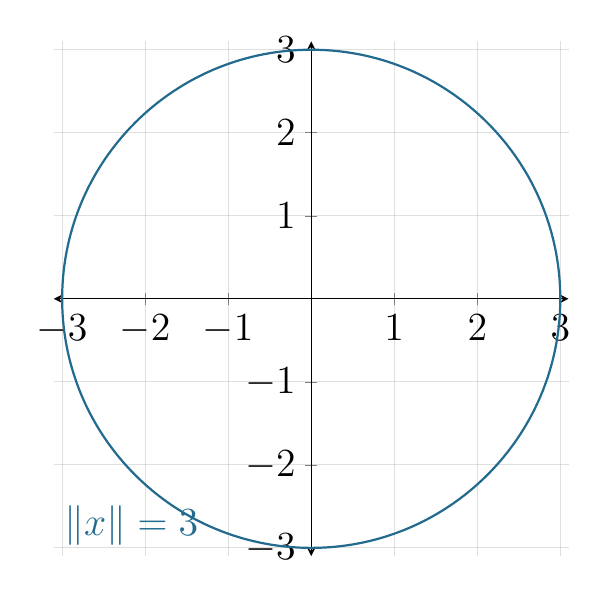
\begin{tikzpicture}[>=stealth, scale=1]
		\begin{axis}[xmin = -3.1, xmax=3.1, ymin=-3.1, ymax=3.1,axis x line=middle, axis y line=middle, axis line style=<->, xlabel={}, ylabel={}, grid=both, grid style = {opacity=.5}, x=30pt, y=30pt]
			\draw[BLUE_E, thick,radius=90pt] (axis cs:0,0) circle node[pos=0, above right] {$\Vert x \Vert = 3$};
		\end{axis}
	\end{tikzpicture}
	
	% exe:milieu-segment
	% page 10
	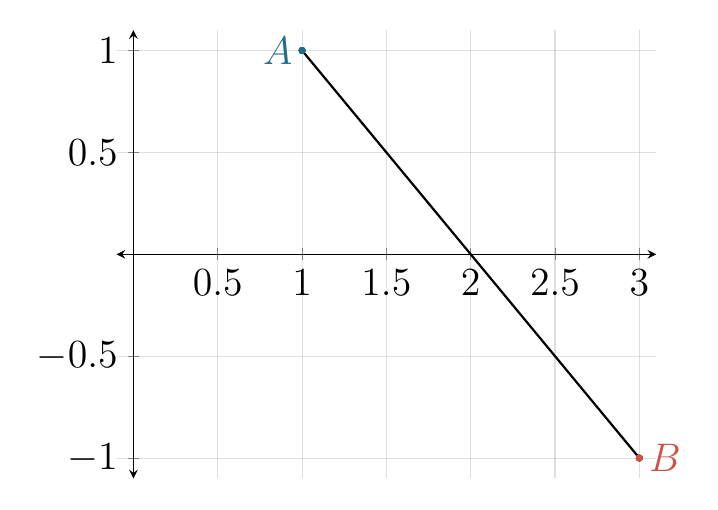
\begin{tikzpicture}[>=stealth, scale=1]
		\begin{axis}[xmin = -0.1, xmax=3.1, ymin=-1.1, ymax=1.1,axis x line=middle, axis y line=middle, axis line style=<->, xlabel={}, ylabel={}, grid=both, grid style = {opacity=.5}]
			\addplot[BLUE_E, mark=*, mark size = 1] (1,1) node[left] {$A$};
			\addplot[RED_E, mark=*, mark size = 1] (3,-1) node[right] {$B$};
			\draw[-, thick] (axis cs:1,1) -- (axis cs:3,-1);
		\end{axis}
	\end{tikzpicture}
%
\end{document}